\documentclass[a4paper,oneside,12pt]{report}


\usepackage[utf8]{inputenc}
\usepackage[T1]{fontenc}
\usepackage[ngerman]{babel}
\usepackage{graphicx}
\usepackage{setspace}

\graphicspath{ {./Images/} }


%Adjust the page margins 
\usepackage[left=3cm, right=3cm, top=2cm, bottom=2cm, a4paper, portrait]{geometry}

%For fancy headers and footers
\usepackage{fancyhdr}
\usepackage{mathpazo}
%Change captions
\usepackage[font=footnotesize,labelfont=bf,tableposition=top]{caption}
%Enable link support in the pdf
\usepackage{hyperref}
%Using BibLaTeX (replacing BibTeX)
\usepackage[autostyle,german=guillemets]{csquotes}
\usepackage[natbib=false,citestyle=numeric-comp,bibstyle=numeric-comp,sortcites=true,backend=biber]{biblatex}
\bibliography{template_advanced_thesis_references}


%Adjust headings and footers --> \usepackage{fancyhdr}
%Give the headings some space
\setlength{\headheight}{15pt}
%This is valid for all pages exept chapters
\pagestyle{fancy}
\fancyhf{} % clear all headers and footers
\rhead[\thepage]{{\leftmark}}
\rfoot[{\leftmark}]{\thepage}
\renewcommand{\headrulewidth}{0.4pt}
% For \chapters \maketitle
\fancypagestyle{plain}{%
	\fancyhf{} % clear all header and footer fields
	\rfoot[{\leftmark}]{\thepage}%
	\renewcommand{\headrulewidth}{0pt}
	\renewcommand{\footrulewidth}{0pt}
}




%Adjust hyperlink behavior -> \usepackage{hyperref}
\hypersetup{
	%bookmarks=true,        										 % show bookmarks bar?
	unicode=false,         											 % non-Latin characters in Acrobatics bookmarks
	pdftoolbar=true,      											 % show Acrobatics toolbar?
	pdfmenubar=true,       											 % show Acrobatics menu?
	pdffitwindow=false,     										 % window fit to page when opened
	pdfstartview={FitH},   											 % fits the width of the page to the window
	pdftitle={FWP Grundlagen der kuenstlichen Intelligenz},    		 % title
	pdfauthor={Philipp Muhr, Michael Mican, Maximilian Anzinger}, 	 % author
	pdfsubject={Ampelphasenerkennung},    							 % subject of the document
	pdfkeywords={Kuenstliche Intelligenz, Informatik}, 				 % list of keywords
	pdfnewwindow=true,     											 % links in new window
	colorlinks=true,        										 % false: boxed links; true: colored links
	linkcolor=black,       											 % color of internal links
	citecolor=black,      											 % color of links to bibliography
	filecolor=black,      											 % color of file links
	urlcolor=black        											 % color of external links
}


%Absatzzeilen verhindern
\clubpenalty = 10000
\widowpenalty = 10000 
\displaywidowpenalty = 10000




\begin{document}

	\pagenumbering{alph}  % numbering a, b, c
	\pagenumbering{arabic} % numbering arabic
	
\begin{titlepage}
	\begin{center}
		
		\textsc{\scshape \huge Prüfungsstudienarbeit (PStA)}\\
		\rule{1\textwidth}{1mm} \\[0.5cm]
		{ \LARGE  {\bfseries Technische Hochschule Deggendorf}}\\[0.5cm]
		{ \LARGE   Fakultät Elektrotechnik, Medientechnik und Informatik}\\[0.5cm]
		\rule{1\textwidth}{1mm} \\[4cm] 
		{ \Large \bfseries Thema: Ampelphasenerkennung}\\[2cm]
		{ Fach: FWP Grundlagen der künstlichen Intelligenz}\\[5cm]
		
		\begin{minipage}{0.4\textwidth}
			\begin{flushleft} \normalsize
				\emph{vorgelegt von:}\\[0.3cm]
				Philipp Muhr, Michael Mican, Maximilian Anzinger\\[0.2cm]
				Deggendorf,  \today
			\end{flushleft}
		\end{minipage}
		\begin{minipage}{0.5\textwidth}
			\begin{flushright} \normalsize
				\emph{Prüfer:}\\[0.3cm]
				Prof. Dr. Andreas \textsc{Fischer}\\[0.2cm]
			\end{flushright}
		\end{minipage}\\[2cm]
		{\large \today}
				
	\end{center}
\end{titlepage}

	
	%Inhaltsverzeichnis
	\tableofcontents
	\cleardoublepage
	
	
	\chapter*{Einleitung}
	%Link zu den Kapiteln inkl. Inhaltsverzeichnis
	\addcontentsline{toc}{chapter}{Einleitung}
	\begin{onehalfspace}
		Im Straßenverkehr finden sich viele Herausforderungen. Es müssen viele Situationen vorausgesehen werden, um eine sichere Fahrt zu gewährleisten. Bei immer höher werdenden Verkehrsaufkommen werden es die Fahrer auch in Zukunft nicht einfach haben. Damit die Verkehrssituation sicherer gestaltet werden kann, werden Unmengen an verschiedenen Fahrassistenzsystemen entwickelt. Diese Studienarbeit behandelt ein Assistenzsystem zur leichteren Ampelphasenwahrnehmung. Eine rote Ampel wird schnell übersehen, daher muss auch in dieser Thematik unterstützte Wahrnehmung begünstigt werden. Es soll ein neuronales Netz trainiert werden, das Ampeln und deren unterschiedlichen Schaltphasen (rot, rot-gelb, gelb und grün) erkennen kann. Ziel dieser künstlichen Intelligenz soll sein, dass Sie den Fahrer durch Statusmeldungen in beispielsweise dem Bordmonitor mit der aktuellen Ampelphase informiert. Falls die Sicht des Mobilisten eingeschränkt ist und dieser die Phasen der Ampel nur schwer bis gar nicht erkennen kann soll er sich auf die Anzeige der Ampelerkennung im Bordmonitor verlassen können. Diese Arbeit wird Aufschluss geben, wie die künstliche Intelligenz aufgebaut und trainiert wurde. Außerdem werden unterschiedliche Verfahren im Bereich Image processing beschrieben, um eventuell performantere Ergebnisse zu erzielen. Im ersten Kapitel wird dargelegt, auf welchem neuronalen Netz aufgebaut wurde und wie dieses angelegt wurde.
	\end{onehalfspace}

	\chapter*{Netzwerk}
	\addcontentsline{toc}{chapter}{Netzwerk}
	\begin{onehalfspace}
		Wie bereits erwähnt soll die Erkennung der Ampel bzw. weiterführend die Phase dieser durch ein neuronales Netz realisiert werden.\\
		Mittlerweile gibt es viele verschiedene Neuronale Netze zur Erkennung von Objekten in Bildern und/oder Videos (Object Recognition). Als Basis dient hier meist ein sog. Convolutional Neural Network (CNN) welches aus mehreren namensgebenden Convolutional Layern, Pooling Layern, einem Fully Connected Layer und einer Softmax Funktion besteht.
		Dieses Konzept wird dann um verschiedene Operatoren, Funktionen oder Ähnliches erweitert.\\
		Im Nachfolgenden wird das, von uns genutzte, Netzwerk YoloV3-tiny genauer erklärt bzw. allgemein auf das Konzept von YOLO eingegangen.
		\section*{YOLO}
		\subsection*{Yolo allgemein}
		YOLO ist laut offizieller Aussage ein "`Echtzeit Objekterkennungs System"
		\footnote{"https://pjreddie.com/darknet/yolo/", besucht am 30.05.2020 (eigene Übersetzung)},
		welches vorallem auf Geschwindigkeit bei trotzdem gut bleibender Genauigkeit setzt.\\
		YOLO nutzt im Gegensatz zu vielen herkömmlichen Objekterkennungsnetzen (wie z.B. Faster-RCNN oder Mask-RCNN) nicht mehrerer Netze hintereinander, bei dem z.B. das erste durch ein sog. Region Proposal Network dargestellt wird (welches interessante Regionen herausfiltert), sondern geht "`einen völlig anderen Weg und schaut nur ein einziges Mal auf das Bild"
		\footnote{"https://www.sigs-datacom.de/trendletter/2018-10/4-wie-man-in-echtzeit-mehrere-objekte-mit-deep-learning-und-yolo-erkennen-und-klassifizieren-kann.html", besucht am 30.05.2020}
		und "`erkennt gleichzeitig alle interessanten Bereiche und klassifiziert diese mit eine[m] Score"
		\footnote{"https://www.sigs-datacom.de/trendletter/2018-10/4-wie-man-in-echtzeit-mehrere-objekte-mit-deep-learning-und-yolo-erkennen-und-klassifizieren-kann.html", besucht am 30.05.2020}\\
		Diese Technik ermöglicht es dem Netzwerk eine deutlich schneller Klassifizierung vorzunehmen. \clearpage
		Jedoch bringt diese Geschwindigkeit bzw. diese Technik auch einen Nachteil mit sich. Für ein solches Model ist es schwieriger ein sehr kleines Objekt zu erkennen, da das Grid welches auf das Bild gelegt wird sehr "grob"\space im Vergleich zu anderen Netzen ist. \\
		Deshalb ist ein Model wie z.B. Retinanet mit einem Backbone wie einem FPN deutlich besser in der Erkennung von kleinen Objekten bzw. auch in der Genauigkeit der Vorhersagen generell, auch wenn dies natürlich Performance kostet. (vgl. Abbildung 1
		\footnote{"https://syncedreview.com/2018/03/27/the-yolov3-object-detection-network-is-fast/", besucht am 30.05.2020})\\
		\begin{figure}[h!]
			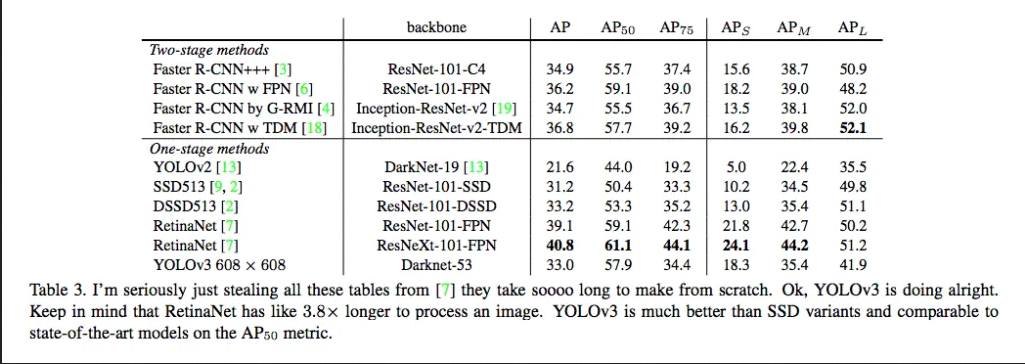
\includegraphics[width=\linewidth]{Comparison.png}
			\caption{"`Yolov3 Comparison"}
			\label{fig:comparison}
		\end{figure}
		\subsection*{YoloV3-tiny}
		Für unseren Einsatzfall lohnt es sich, wie oben beschrieben, einen Blick auf Tiny Yolo zu werfen. \\
		Ein "`ganzes"\space YOLO Netzwerk wie z.B. das neue YoloV4 oder das gängige YoloV3 Model bieten gute Ergebnisse, jedoch ist die Performance dieser auf einem Nvidia Jetson Nano Gerät leider zu schlecht, um diese dem Nutzer direkt "`live"\space weitergeben zu können.
		Daher wird eine "`kleine"\space Version von Yolo (genannt Tiny-Yolo) für diesen Anwendungsfall genutzt. Tiny-Yolo (V3) kann Bilder auf einem Nvidia Jetson Nano mit ca. 25 Bildern pro Sekunde klassifzieren und bietet somit eine, für diese Platform, sehr gute Performance.\clearpage
		Aufgrund dieser deutlich höheren Performance (ca. 6,2x die Geschwindigkeit von YoloV3-416) verschlechtert sich die Genauigkeit jedoch auch um ca. 40\% (vgl. Abbildung 2)\\
		\begin{figure}[h!]
			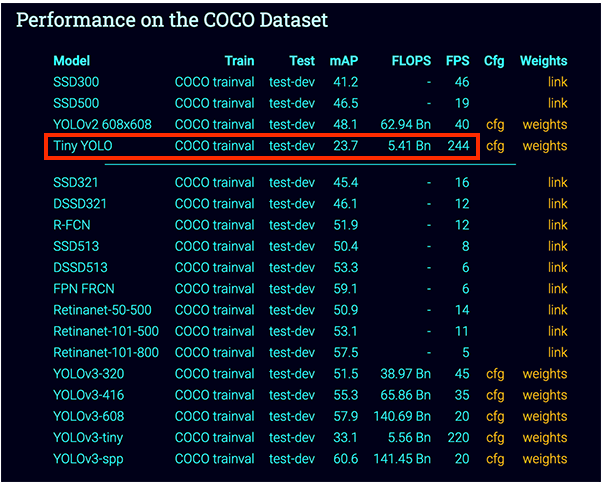
\includegraphics[scale=0.7]{YoloV3-tiny.png}
			\caption{"`Yolov3(-tiny) Comparison"}
			\label{fig:yolov3-tiny}
		\end{figure}
	\end{onehalfspace}
	\chapter*{Realisierung}
	\addcontentsline{toc}{chapter}{Realisierung}
	\begin{onehalfspace}
		Wie schon in der vorherigen Sektion erwähnt, soll das Projekt auf einem Nvidia Jetson Nano realisiert werden. Dieser bietet für seinen vergleichsweise niedrigen Preis (ca. 99\$
		\footnote{"https://nvidianews.nvidia.com/news/nvidia-announces-jetson-nano-99-tiny-yet-mighty-nvidia-cuda-x-ai-computer-that-runs-all-ai-models", besucht am 31.05.2020})
		im Hinblick auf Inferenz eine sehr gute Performance für die Kosten.
		\subsection*{Hardware}
		Der Nvidia Jetson Nano berechnet mit seiner 128 Kern Nvidia Maxwell Grafikeinheit und seinem Quad-Core ARM Cortex -A57 laut Nvidia 472 GFLOPs.
		\footnote{"https://developer.nvidia.com/embedded/develop/hardware", besucht am 31.0.5.2020}
		Das Gerät wird für unseren Anwendungsfall zusätzlich mit einer Raspberry Pi Camera v2.1 ausgestattet, welche den Videostream liefert. Das Nvidia System ermöglicht eine Video Dekodierung von bis zu vier gleichzeitigen Full-HD Streams bei 30 Bildern pro Sekunde bzw. analog von acht bei 30 Bildern pro Sekunde.
		\footnote{"https://developer.nvidia.com/embedded/develop/hardware", besucht am 31.0.5.2020}
		\subsection*{Software}
		Nvidia schafft es bei der Jetson Platform die Geräte sehr gut zu optimieren bzw. die Hardware optimal zu nutzen. Dies ermöglichen Frameworks wie z.B. Deepstream und/oder TensorRT
		\subsubsection*{Deepstream}
		Deepstream ist ein Software Development Kit, das "`ein beschleunigtes AI Framework darstellt, welches zur Erstellung von Intelligenten Video Analyse Pipelines genutzt wird."
		\footnote{"https://docs.nvidia.com/metropolis/deepstream/dev-guide/", besucht am 31.05.2020 (eigene Übersetzung)}
		Deepstream fungiert als "`Schnittstelle" zwischen Python, C, C++ Applikationen und der Platform selbst (z.B. einem Nvidia Jetson Nano / TX2).
		Weiterführend basiert es auf CUDA (einer GPU basierten parallelen Programmiersprache welche oft bei neuronalen Netzen zum Einsatz kommt) welches TensorRT nutzt.
		\subsubsection*{TensorRT}
		TensorRT ist, analog zu Deepstream, auch ein Software Development Kit, welches für "high-performance deep learning inference"
		\footnotetext{"https://developer.nvidia.com/tensorrt", besucht am 31.05.2020} genutzt werden kann.
		Applikationen die auf TensorRT basieren können bis zu 40 mal schneller sein als vergleichbare Applikation, welche auf einem CPU berechnet werden.
		\footnotetext{"https://developer.nvidia.com/tensorrt", besucht am 31.05.2020}
		Dieses SDK konvertiert ein trainiertes Neuronales Netzwerk mithilfe eines TensorRT Optimizers in eine TensorRT Runtime Engine. Dies geschieht durch die Kombinierung von Layern und optimierung der Kernel Auswahl.
		\footnotetext{"https://docs.nvidia.com/deeplearning/tensorrt/developer-guide/index.html"}
		Durch diese Umwandlung bzw. Optimierung des Netzwerkes kann ein enormer Geschwindigkeitsgewinn , wie oben beschrieben, erzielt werden.
	\end{onehalfspace}
	\chapter*{Labeling}
	\addcontentsline{toc}{chapter}{Labeling}
	\begin{onehalfspace}
		Labeling
	\end{onehalfspace}
	\chapter*{Data Preprocessing}
	\addcontentsline{toc}{chapter}{Data Preprocessing}
	\begin{onehalfspace}
		Data Preprocessing
	\end{onehalfspace}
	\chapter*{Image Processing}
	\addcontentsline{toc}{chapter}{Image Processing}
	\begin{onehalfspace}
		Image Processing
	\end{onehalfspace}
	\chapter*{Data augmentation}
	\addcontentsline{toc}{chapter}{Data Augmentation}
	\begin{onehalfspace}
		Data Augmentation
	\end{onehalfspace}
	\chapter*{Probleme}
	\addcontentsline{toc}{chapter}{Probleme}
	\begin{onehalfspace}
		Probleme
	\end{onehalfspace}
	\chapter*{Schlusswort}
	\addcontentsline{toc}{chapter}{Schlusswort}
	\begin{onehalfspace}
		Schlusswort
	\end{onehalfspace}
	
\end{document}
